\documentclass{beamer}
\usepackage[utf8]{inputenc}
\usepackage[brazil]{babel}
\usepackage{xcolor}
\usepackage{tikz}
\usetikzlibrary{positioning,calc}
\usepackage{graphicx}
\usepackage{cite}
\usepackage{hyperref}
\usepackage{array}
\usepackage{amsmath}
\usepackage{amssymb}
\usepackage{amsthm}
\usepackage{listings}
\usepackage{fontawesome}
\usepackage{caption}
\usepackage{subcaption}
\usepackage{wrapfig}
\usetheme{mtmufsc} %%%%%%%%Use this template
\renewcommand{\qedsymbol}{$\blacksquare$}
\usepackage[alf]{abntex2cite}


% This is a beamer template inspired by unofficial Oxford University Beamer Template, made by Clara Eleonore Pavillet.
\title{O poder da Aprendizagem Profunda}
\author{Felipe Kaminsky Riffel}
\date{\today}
\institute{Universidade Federal de Santa Catarina}

\begin{document}

{\setbeamertemplate{footline}{} 
\frame{\titlepage}}
% \frame{}

\begin{frame}{Sumário}
    \tableofcontents
\end{frame}
  
% %Sempre que iniciar uma nova sessão, você pode fazer um slide de transição com o índice.
% \begin{frame}
% \tableofcontents[currentsection]
% \end{frame}

\section{Artigo: Why does deep and cheap learning work so well?}    
\begin{frame}
\tableofcontents[currentsection]
\end{frame}

\begin{frame}{Why does deep and cheap learning work so well?}

Artigo: \\

LIN, Henry W.; TEGMARK, Max; ROLNICK, David. Why does deep and cheap learning work so well? Journal of Statistical Physics, v. 168, n. 6, p. 1223–1247, 2017.

\end{frame}

\subsection{Introdução}
\begin{frame}
    \tableofcontents[currentsection]
\end{frame}


\begin{frame}{Introdução}

Três problemas principais da teoria de redes neurais: \\

\begin{itemize}
    \item Expressabilidade: que funções podemos expressar? \pause \\
    \item Eficiência: quão complexa a rede tem que ser? \pause \\
    \item "Aprendibilidade": quão rápido a rede consegue aprender a ajustar os bons parâmetros? \footnote[frame]{Traduzido de "Learnability"} \pause
\end{itemize}

Aqui, focamos nos dois primeiros: \textbf{Expressabilidade} e \textbf{Eficiência}.
\end{frame} 

\begin{frame}{Introdução}
    Problema: "como redes neurais funcionam bem na prática, se o número de funções possíveis é exponencialmente maior que o número de redes possíveis?"

\end{frame}


\begin{frame}{Introdução}

    \textbf{Exemplo:} imagem preta/branca de 1MP ~ vetor de 1000000 entradas com 256 valores possíveis (valor em cada pixel)

    \pause

    \begin{columns}
        \begin{column}{0.3\textwidth}
            \begin{figure}
                
\includegraphics[width=\textwidth]{fig/keyboard-cat.png}
            \end{figure}
        \end{column}
        \begin{column}{0.1\textwidth}
            \[
                \iff
            \]
        \end{column}
        \begin{column}{0.3\textwidth}
            \small
            \[
                \begin{pmatrix}
                    x_1 \\
                    \vdots \\
                    x_{1000000}
                \end{pmatrix}
            \]
            \[
            x_i \in I_{256} := \{1,2,3,\dots,256\}
            \]
        \end{column}
    \end{columns}

    \pause

    \vspace{1em}

    Nº total de imagens possíveis: $256^{1000000}$.

    \pause
    \vspace{1em}

    Se existe $p: I_{256} \to (0,1)$ que associa cada imagem a uma probabilidade, p deve ter uma lista $256^{1000000}$ valores (!!!)
\end{frame}

\begin{frame}
    Porém, redes neurais relativamente simples conseguem calcular bem a tarefa.
    
    \small

    \begin{columns}
        \begin{column}{0.3\textwidth}
            \begin{figure}
                
\includegraphics[width=\textwidth]{fig/keyboard-cat.png}
            \end{figure}
        \end{column}
        \begin{column}{0.3\textwidth}
            \begin{figure}
                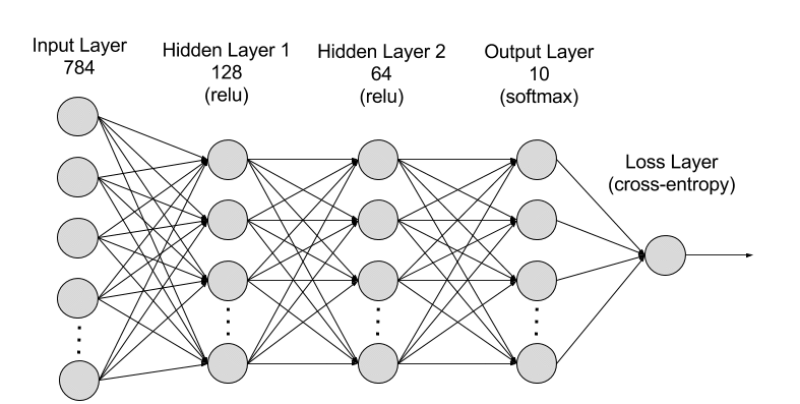
\includegraphics[width=\textwidth]{fig/nn.png}
            \end{figure}
        \end{column}
        \begin{column}{0.3\textwidth}
            \[
                p(\text{Gato} |\bf{x}) = 83\%
            \]
        \end{column}
    \end{columns}
    
    \vspace{1em}

    \pause

    A \textbf{matemática} ajuda a explicar: as redes neurais conseguem diminuir drasticamente a explosão combinatória de número de parâmetros em relação ao número de valores;
    \vspace{1em}
    
    \pause

    A razão também é \textbf{física}: as leis sugerem que os datasets de interesse são, em sua maioria, advindos de distribuições simples.

\end{frame}


\subsection{Expressabilidade e Eficiência de Redes Rasas}
\begin{frame}
    \tableofcontents[currentsection]
\end{frame}

\begin{frame}{Redes neurais}

    Considere $\mathbf x \in \mathbb R^d$. Sejam $A_i:\mathbb R^d \to \mathbb R^d$ operadores afim, i.e.,

    \[
        A_i = W_i - b_i
    \]
    com $W_i \in \mathbb R^{m_i \times n_i}$ e $b_i \in \mathbb R^{n_i}$.

    \vspace{1em}

    \pause 

    Dadas $\sigma_i:\mathbb R^{n_i} \to \mathbb R^{m_i}$ não linear, chamamos de rede neural feedforward uma função $\mathbf f: \mathbb R^n \to \mathbb R^m$ da forma:

    \begin{equation}
        \mathbf f (\mathbf x) = \sigma_n A_n \dots \sigma_2 A_2 \sigma_1 A_1 \mathbf x.
    \end{equation}

\end{frame}

\begin{frame}{Redes neurais}
    $\mathbf \sigma_i$ pode ser qualquer operador não linear. Escolhas comuns são, dado $\mathbf x = (x_1, \dots, x_n)$:

    \begin{itemize}
        \item Função local: escolha $\sigma : \mathbb R \to \mathbb R$ não linear e aplique ponto a ponto $\mathbf \sigma_i(\mathbf x) = (\sigma(x_1),\dots,\sigma(x_n))$; \pause \\
        \item Max-pooling: $\sigma_i (\mathbf x) = \max_{j=1,\dots,n} (x_j)$; \pause \\
        \item Softmax: \[
            \sigma_i(\mathbf x) = \frac{1}{\sum_{j=1}^n e^{x_j}}(e^{x_1}, \dots, e^{x_n}). 
        \]
    \end{itemize}

\end{frame}

\begin{frame}{Teorema 1 (Aproximação da multiplicação)}
    Seja $\mathbf f$ rede neural da forma $\mathbf f (\mathbf x) = A_2 \sigma A_1\mathbf x$, onde $\mathbf \sigma$ é aplicação não linear ponto a ponto qualquer. Considere as camadas de entrada, escondida e de saída com tamanhos 2, 4 e 1 respectivamente. Então, $\mathbf f$ pode aproximar uma porta de multiplicação arbitrariamente bem.

    Ou seja, dado $\varepsilon>0$, para qualquer $\sigma$ não linear (aplicada ponto a ponto), existem  $A_1:\mathbb R^2 \to \mathbb R^4, A_2:\mathbb R^4 \to \mathbb R$ tais que a rede $f(x) = A_2 \sigma A_1 \mathbf{x}$ é tal que, dado $x=(u \; v)^T$ qualquer

    \[
        |f(x) - uv|<\varepsilon
    \]

    para $u,v$ em um compacto qualquer.

\end{frame}

\begin{frame}{Teorema 1 - Demonstração}
    \small
    Seja $\sigma:\mathbb R \to \mathbb R$ não linear qualquer suficientemente suave. Na expansão de Taylor em torno de $x=0$:

    \[
        \sigma(u) = \sigma(0) + \sigma'(0)u + \frac{u^2}{2} \sigma''(0) + \mathcal O(u^3).
    \]

    Sem perda de generalidade, considere $\sigma''(0) \neq 0$ (ou então, ajuste $b_1$ para que $\sigma''(A_{1,1}x-b_{1,1}),\sigma''(A_{1,2}x-b_{1,2})\neq0$, que deve existir dado que é não linear). 

    \vspace{1em}
    \pause

    Então,

    \begin{align*}
        m(u,v) &:= \frac{\sigma(u+v)+\sigma(-u-v)-\sigma(u-v)-\sigma(v-u)}{4\sigma''(0)} \\ 
        &= \sigma''(0) \frac{(u+v)^2 + (-u-v)^2 - (u-v)^2 - (v-u)^2  + \mathcal O((u+v)^3)}{4\sigma''(0)}  \\
        &= uv + \mathcal O((u+v)^3)
    \end{align*}
\end{frame}


\begin{frame}{Teorema 1 - Demonstração}
    \small
    Ou seja, $m(u,v) = uv + \mathcal O((u+v)^3)$, de modo que $\lim_{u^2+v^2 \to 0} \frac{m(u,v)-uv}{u^2+v^2} = 0$. 
    
    \pause

    Veja que, $m(u,v) = A_2 \sigma A_1 (u \; v)^T$, onde:

    \begin{equation*}
        A_1 = \begin{pmatrix}
            1 & 1 \\
            -1 & -1 \\
            1 & -1 \\
            -1 & 1
        \end{pmatrix},
        A_2 = (4\sigma''(0))^{-1} \begin{pmatrix}
            1 & 1 & -1 & -1
        \end{pmatrix}.
    \end{equation*}

    \pause
    \vspace{1em}

    Taylor fornece uma estimativa local, sendo boa para $u,v \approx 0$. Para $u,v$ num compacto de raio qualquer, tome $\lambda A_1$ e $\lambda^{-2}A_2$ na definição de $\mathbf f$, de modo a obter
    \begin{align*}
        f(x) = (\lambda^{-2}A_2)\sigma(\lambda A_1)x = \lambda^{-2} ( \lambda u \lambda v) = uv,
    \end{align*}
    tornando a estimativa tão boa quanto se queira. $\square$
\end{frame}


\begin{frame}{Teorema 1 - Comentário}
    \begin{figure}
        \caption{Ilustração da arquitetura da rede no teorema anterior}
        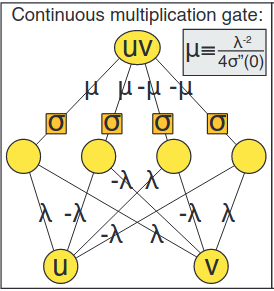
\includegraphics[width=0.5\textwidth]{fig/productgate.png}
        \caption*{Fonte: Lin, et.al. (2017)}
    \end{figure}
\end{frame}

%\subsection{Interpretações físicas}
%\begin{frame}{Probabilidade condicional}
%
%    Considere $p:X \to (0,1)$ uma distribuição de probabilidade sobre um espaço X. A probabilidade condicional: 
%
%    \begin{equation}
%        p(\bf{x}|y) = \frac{p(\bf{x}\cup y)}{p(y)}
%    \end{equation}
%
%    \begin{itemize}
%        \item $\bf{x}$ varia no espaço amostral;
%        \item $y$ é outra variável condicionando, ou um parâmetro do modelo
%    \end{itemize}
%    
%    \pause
%
%    \textbf{Exemplos}:
%
%    \begin{itemize}
%        \item $\bf x$ é o vetor de pixels da imagem e $y$ é um elemento de um conjunto de animais \{Gato, Cachorro, Coelho, etc.\};
%        \item $\bf x$ é a magnetização em cada parte de uma barra de metal, $y$ é um elemento de um conjunto de elementos \{Ferro, Alumínio, etc.\}
%    \end{itemize}
%
%\end{frame}
%
%\begin{frame}{Teorema de Bayes}
%    
%    Calcular $p(\mathbf{x}|y)$ é conhecido como problema de \textbf{predição}, e $p(y|\mathbf x)$ de \textbf{classificação}.
%    \vspace{1em}
%
%    \pause
%    
%    Para calcular $p(y| \mathbf x)$, usamos o \textbf{Teorema de Bayes}:
%
%    \begin{align*}
%        p(y|\mathbf x) &= \frac{p(\mathbf{x}|y)p(y)}{\sum_{y' \in Y}p(\mathbf{x}|y')p(y')}
%        
%        &\left( = \frac{p(\mathbf{x}|y)p(y)}{p(\mathbf{x})} \right)
%    \end{align*}
%    
%
%    \begin{itemize}
%        \item $p(y)$ é chamada informação a priori;
%    \end{itemize}
%\end{frame}

\section{Referências}
\begin{frame}
\tableofcontents[currentsection]
\end{frame}

\begin{frame}
\frametitle{Referências}
\vspace{-2em}
\scriptsize
\bibliographystyle{abntex2-alf}
\bibliography{refs.bib}    
\end{frame}

\begin{frame}

\begin{center}
\Large Obrigado!
\end{center}

\vspace{1em}
Contato: riffel.felipe@grad.ufsc.br 

Repositório com os experimentos desenvolvidos: https://github.com/felipekriffel/TCC-Regularizacao-EIT
    
\end{frame}

\end{document}

